\documentclass[crop, tikz, border=0pt]{standalone}
\usepackage{esvect}
\usetikzlibrary{bayesnet}
%\usepackage{color}
\begin{document}
%\color{white}
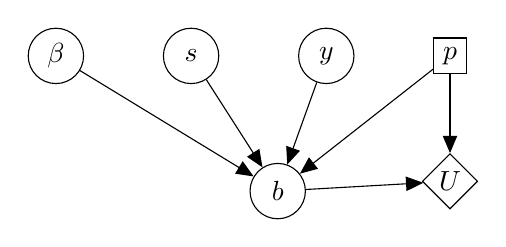
\begin{tikzpicture}%[draw=black]
\begin{scope}[xscale=1]

%\node[det] (alpha) {$\alpha$} ; %
\node[latent] (beta) {$\vv \beta $} ; 
\node[latent, right=of beta] (scratched) {$s$};
\node[latent, right=of scratched] (year) {$y$};
\node[shape=rectangle, draw=black, right=of year] (price) {$p$};
\node[det, below=of price] (utility) {$U$};
\node[latent, below=of scratched, xshift=1.1cm] (bought) {$b$};

\edge {beta} {bought} ; %
\edge {scratched} {bought} ; %
\edge {year} {bought} ; %
\edge {price} {bought} ; %
\edge {bought} {utility} ; %
\edge {price} {utility} ; %
\end{scope}

\end{tikzpicture}
\end{document}

